\documentclass[tikz,border=6pt]{standalone}
\usepackage{tikz}
\usetikzlibrary{arrows.meta,positioning,calc,fit,backgrounds}
\begin{document}
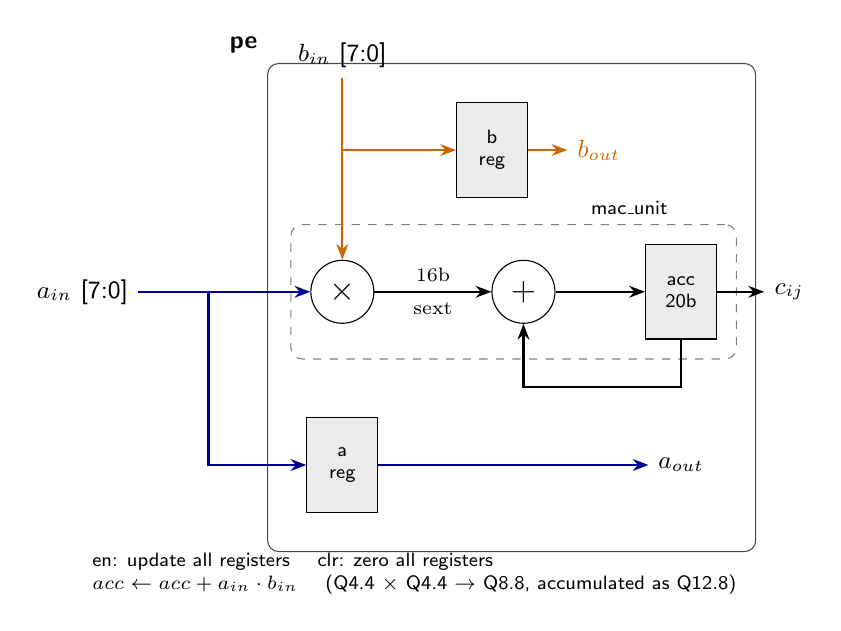
\begin{tikzpicture}[font=\sffamily\small, >={Stealth[length=2mm]},
  reg/.style={draw, fill=gray!15, minimum width=9mm, minimum height=12mm, align=center, font=\sffamily\scriptsize},
  op/.style={draw, circle, minimum size=8mm, fill=white, font=\large}]
\node (ain) at (0,0) {$a_{in}$ [7:0]};
\node (bin) at (3.3,3.0) {$b_{in}$ [7:0]};
\node[op] (mul) at (3.3,0) {$\times$};
\node[op] (add) at (5.6,0) {$+$};
\node[reg] (acc) at (7.6,0) {acc\\20b};
\node[reg] (areg) at (3.3,-2.2) {a\\reg};
\node[reg, rotate=0] (breg) at (5.2,1.8) {b\\reg};
\node (aout) at (7.6,-2.2) {$a_{out}$};
\node (bout) at (5.2,-3.7) {};
\draw[->, thick, blue!60!black] (ain) -- (mul);
\draw[->, thick, blue!60!black] (1.6,0) |- (areg);
\draw[->, thick, blue!60!black] (areg) -- (aout);
\draw[->, thick, orange!80!black] (bin) -- (mul);
\draw[->, thick, orange!80!black] (3.3,1.8) -- (breg);
\draw[->, thick, orange!80!black] (breg.east) -- ++(0.5,0) node[right]{$b_{out}$};
\draw[->, thick] (mul) -- node[above,font=\scriptsize]{16b} node[below,font=\scriptsize]{sext} (add);
\draw[->, thick] (add) -- (acc);
\draw[->, thick] (acc.east) -- ++(0.6,0) node[right]{$c_{ij}$};
\draw[->, thick] (acc.south) -- ++(0,-0.6) -| (add.south);
\node[font=\sffamily\scriptsize, align=left, anchor=north west] at (0,-3.2)
  {en: update all registers \quad clr: zero all registers\\
   $acc \leftarrow acc + a_{in}\cdot b_{in}$ \quad (Q4.4 $\times$ Q4.4 $\to$ Q8.8, accumulated as Q12.8)};
\begin{scope}[on background layer]
\node[draw=black!50, dashed, rounded corners, fit=(mul)(add)(acc), inner sep=7pt,
      label={[font=\sffamily\scriptsize]above right:mac\_unit}] {};
\node[draw=black!70, rounded corners, fit=(mul)(acc)(areg)(breg), inner sep=14pt,
      label={[font=\sffamily\small\bfseries]above left:pe}] {};
\end{scope}
\end{tikzpicture}
\end{document}
